\documentclass[conference]{IEEEtran}
\usepackage{booktabs}
\usepackage{graphicx}
\usepackage{amsmath,amssymb}
\usepackage[hidelinks]{hyperref}

\title{Reliability-Aware LSTM-MPC With Dual Witnesses for Sensor-Fault-Tolerant DC-Motor Control: A Preregistered Evaluation}
\author{\IEEEauthorblockN{TODO: author list}
\IEEEauthorblockA{TODO: affiliation \\ TODO: email}}

\begin{document}
\maketitle

\begin{abstract}
TODO: 150--200 words. Frame as a rigorous evaluation of learned
residual-based sensor-fault tolerance for LSTM model-predictive control
of a DC motor: frozen evidence, a post-hoc startup-latch decomposition,
detector fixes (CUSUM anti-windup, warm-up gating, independent-witness
AND rule, bounded recovery), classical baselines with their own
detectors, and a preregistered confirmatory study on fresh seeds. No
claim of general superiority; negative results are retained.
\end{abstract}

\section{Introduction}
\label{sec:intro}
TODO: problem (speed-sensor faults under MPC), why learned residuals,
the startup-latch confound found post-hoc, contributions:
(1)~decomposition separating false latch from missed detection;
(2)~V4 detector variants with frozen-compatible defaults;
(3)~classical baselines with independent detectors;
(4)~preregistered confirmatory protocol on fresh seeds/blocks.

\section{Related Work}
\label{sec:related}
TODO: learned models for MPC \cite{Mayne2000}; LSTM sequence models
\cite{Hochreiter1997}; CUSUM change detection \cite{Page1954};
observer-based fault diagnosis (TODO: search terms: Luenberger observer
fault detection survey; EKF fault diagnosis review); sensor validation
and plausibility checks (TODO: search terms: analytic redundancy
sensor fault detection survey).

\section{Method}
\label{sec:method}

\subsection{Plant and control law}
TODO: DC-motor model, frozen LSTM-MPC configuration, PI fallback.

\begin{figure*}[t]
\centering
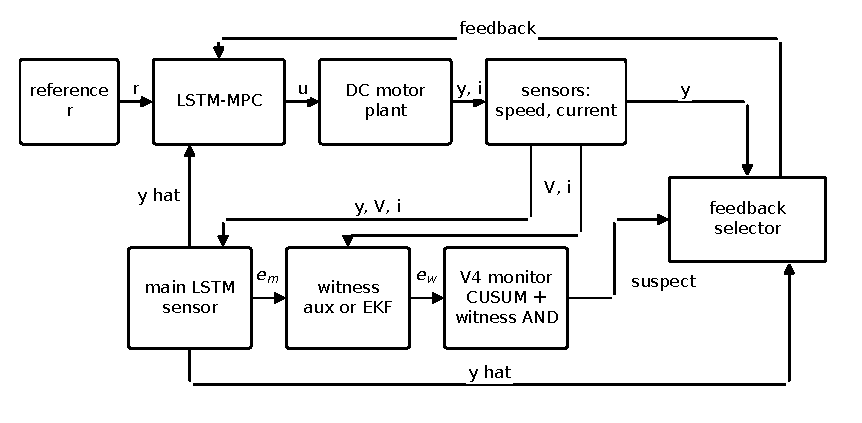
\includegraphics[width=7.16in]{figures/fig_architecture.pdf}
\caption{V4 fault-tolerant loop. The main LSTM virtual sensor and an
independent witness (auxiliary LSTM or EKF, neither consuming measured
speed) feed the V4 monitor, which combines a CUSUM residual test with a
witness-agreement AND rule. Residuals $e_m$ (main) and $e_w$ (witness)
drive entry; the feedback selector substitutes the main estimate while
suspect. No ground-truth signal enters the online path.}
\label{fig:architecture}
\end{figure*}

\subsection{Frozen detector and its failure modes}
TODO: CUSUM structure, startup false-latching (Fig.~\ref{fig:timeline}),
unbounded discharge, load-induced false entry.

\begin{figure}[t]
\centering
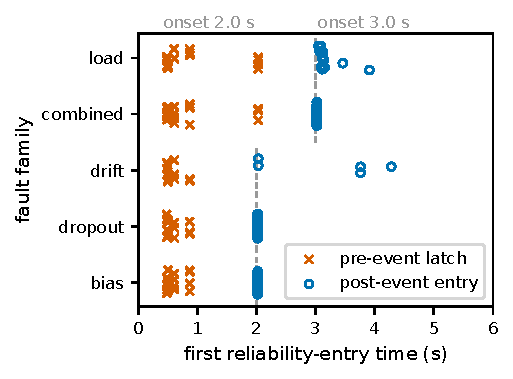
\includegraphics[width=3.5in]{figures/fig_latch_timeline.pdf}
\caption{First reliability-entry times per Part~B C3 fault family
(post-hoc). Crosses: pre-event latches on a healthy sensor (startup
cluster below 1.2~s; one mid-run latch at 2.03~s); circles: post-event
entries. Dashed lines: fault onsets.}
\label{fig:timeline}
\end{figure}

\subsection{V4 detector variants}
TODO: anti-windup clamp, warm-up gating, witness AND rule, bounded
recovery; factorial ablation; frozen-compatible defaults.

\subsection{Classical baselines}
TODO: E2 (EKF+CUSUM), S1 (fixed gate), S2 (median/rate plausibility),
S3 (Luenberger+CUSUM), each with its own detector and substitution.

\section{Experimental Protocol}
\label{sec:protocol}
TODO: V4 dataset (closed-loop + startup-rich, seed 62026), 11 training
seeds, frozen calibration procedures with bootstrap uncertainty,
preregistered seed blocks, confirmatory hypotheses H1--H9 with Holm
correction, clean-start pair-exclusion rule, intention-to-treat tracking
endpoints. Full preregistration: \texttt{V4\_PREREGISTRATION.md}.

\section{Results}
\label{sec:results}

\subsection{Post-hoc decomposition (frozen data)}
The frozen pooled detection endpoint conflates missed detection with
pre-event false latching: conditional on a clean start, C3 detects
11/11 bias faults at 0.02~s (Table~\ref{tab:posthoc}, Fig.~\ref{fig:cond}).

\begin{table}[t]
\centering
\caption{Post-hoc false-latch rate and conditional detection per
training seed (Part~B pooled; exploratory).}
\label{tab:posthoc}
% AUTO-GENERATED by scripts/v4_paper_tables.py
% Provenance: results/v4/posthoc/per_seed_summary.csv (PartB pooled rows, POST-HOC)
% DO NOT EDIT BY HAND; regenerate instead.
\begin{tabular}{lcccc}
\toprule
Training seed & runs & false-latch rate [95\% CI] & clean starts & cond. detection \\
\midrule
2026 & 100 & $0.200$ [0.133, 0.289] & 80 & $0.675$ \\
2027 & 100 & $0.680$ [0.583, 0.763] & 32 & $0.812$ \\
2028 & 100 & $0.000$ [0.000, 0.037] & 100 & $0.670$ \\
\bottomrule
\end{tabular}

\end{table}

\begin{figure}[t]
\centering
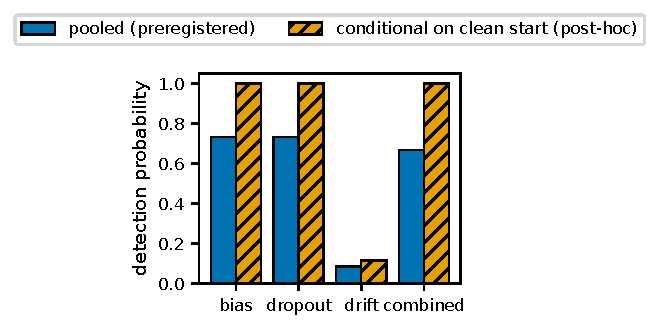
\includegraphics[width=3.5in]{figures/fig_conditional_detection.pdf}
\caption{Pooled preregistered detection vs.\ conditional-on-clean-start
detection by family (post-hoc). Drift remains hard to detect under
either definition.}
\label{fig:cond}
\end{figure}

\begin{table*}[t]
\centering
\caption{Operating envelope: unchanged preregistered labels beside
post-hoc conditional-on-clean-start labels (exploratory; 16 conditions).}
\label{tab:envelope}
% AUTO-GENERATED by scripts/v4_paper_tables.py
% Provenance: results/v4/posthoc/envelope_relabelled_posthoc.csv (POST-HOC)
% DO NOT EDIT BY HAND; regenerate instead.
\begin{tabular}{lllll}
\toprule
Condition & preregistered & latches & cond. detection & post-hoc \\
\midrule
bias\_10pct & LIMITED & 4/15 & $1.00$ & SUPPORTED \\
bias\_15pct & LIMITED & 4/15 & $1.00$ & SUPPORTED \\
bias\_2.5pct & LIMITED & 4/15 & $1.00$ & SUPPORTED \\
bias\_5pct & LIMITED & 4/15 & $1.00$ & SUPPORTED \\
combined\_bias\_15pct\_load\_0.15Nm & LIMITED & 5/15 & $1.00$ & SUPPORTED \\
combined\_bias\_15pct\_load\_0.1Nm & LIMITED & 5/15 & $1.00$ & SUPPORTED \\
combined\_bias\_5pct\_load\_0.15Nm & LIMITED & 5/15 & $1.00$ & SUPPORTED \\
combined\_bias\_5pct\_load\_0.1Nm & LIMITED & 5/15 & $1.00$ & SUPPORTED \\
drift\_10pct & UNSUPPORTED & 4/15 & $0.09$ & UNSUPPORTED \\
drift\_15pct & UNSUPPORTED & 4/15 & $0.18$ & UNSUPPORTED \\
drift\_2.5pct & UNSUPPORTED & 4/15 & $0.09$ & UNSUPPORTED \\
drift\_5pct & UNSUPPORTED & 4/15 & $0.09$ & UNSUPPORTED \\
dropout\_0.1s & UNSUPPORTED & 4/15 & $1.00$ & UNSUPPORTED \\
dropout\_0.5s & LIMITED & 4/15 & $1.00$ & SUPPORTED \\
dropout\_1s & LIMITED & 4/15 & $1.00$ & SUPPORTED \\
dropout\_2s & LIMITED & 4/15 & $1.00$ & SUPPORTED \\
\bottomrule
\end{tabular}

\end{table*}

\subsection{Confirmatory results}
TODO: fill after running Section~9 of the preregistration. Hypothesis
table H1--H9, DET curves, minimum detectable magnitudes, recovery and
robustness summaries, timing distributions.

\begin{table}[t]
\centering
\caption{Frozen Part~B pooled detection anchor (unchanged).}
\label{tab:frozen}
% AUTO-GENERATED by scripts/v4_paper_tables.py
% Provenance: results/final_robustness/detection_wilson_intervals.csv pooled rows (FROZEN)
% DO NOT EDIT BY HAND; regenerate instead.
\begin{tabular}{llll}
\toprule
Family & condition & successes & pooled detection [95\% CI] \\
\midrule
bias & bias\_10pct & 11/15 & $0.733$ [0.480, 0.891] \\
bias & bias\_15pct & 11/15 & $0.733$ [0.480, 0.891] \\
bias & bias\_2.5pct & 11/15 & $0.733$ [0.480, 0.891] \\
bias & bias\_5pct & 11/15 & $0.733$ [0.480, 0.891] \\
combined\_bias\_load & combined\_bias\_15pct\_load\_0.15Nm & 10/15 & $0.667$ [0.417, 0.848] \\
combined\_bias\_load & combined\_bias\_15pct\_load\_0.1Nm & 10/15 & $0.667$ [0.417, 0.848] \\
combined\_bias\_load & combined\_bias\_5pct\_load\_0.15Nm & 10/15 & $0.667$ [0.417, 0.848] \\
combined\_bias\_load & combined\_bias\_5pct\_load\_0.1Nm & 10/15 & $0.667$ [0.417, 0.848] \\
drift & drift\_10pct & 1/15 & $0.067$ [0.012, 0.298] \\
drift & drift\_15pct & 2/15 & $0.133$ [0.037, 0.379] \\
drift & drift\_2.5pct & 1/15 & $0.067$ [0.012, 0.298] \\
drift & drift\_5pct & 1/15 & $0.067$ [0.012, 0.298] \\
dropout & dropout\_0.1s & 11/15 & $0.733$ [0.480, 0.891] \\
dropout & dropout\_0.5s & 11/15 & $0.733$ [0.480, 0.891] \\
dropout & dropout\_1s & 11/15 & $0.733$ [0.480, 0.891] \\
dropout & dropout\_2s & 11/15 & $0.733$ [0.480, 0.891] \\
\bottomrule
\end{tabular}

\end{table}

\section{Limitations}
\label{sec:limitations}
TODO ( retained from frozen evidence, plus V4 scope): drift detection
remains poor; V3 arbitration validated only for single-speed-sensor
faults; current-channel corruption degrades current-fed witnesses;
MPC solve times exceed the control period on the reference machine;
results are simulation-only on one motor model.

\section{Conclusion}
\label{sec:conclusion}
TODO: summary of what the confirmatory study established and did not
establish; no general-superiority claim.

\bibliographystyle{IEEEtran}
\bibliography{references}

\end{document}
